\section{The Design Space of Pipes}
\bjoern{Budget at most 1.5 columns for this section

 There still some redundancy with the related work section, too}
By using different types and topologies of pipes and inserting different media into the completed pipes, a variety of inputs and outputs can be located at arbitrary points on the surface of a 3D print.  We describe the space below.

\begin{figure}[h!]
\centering
    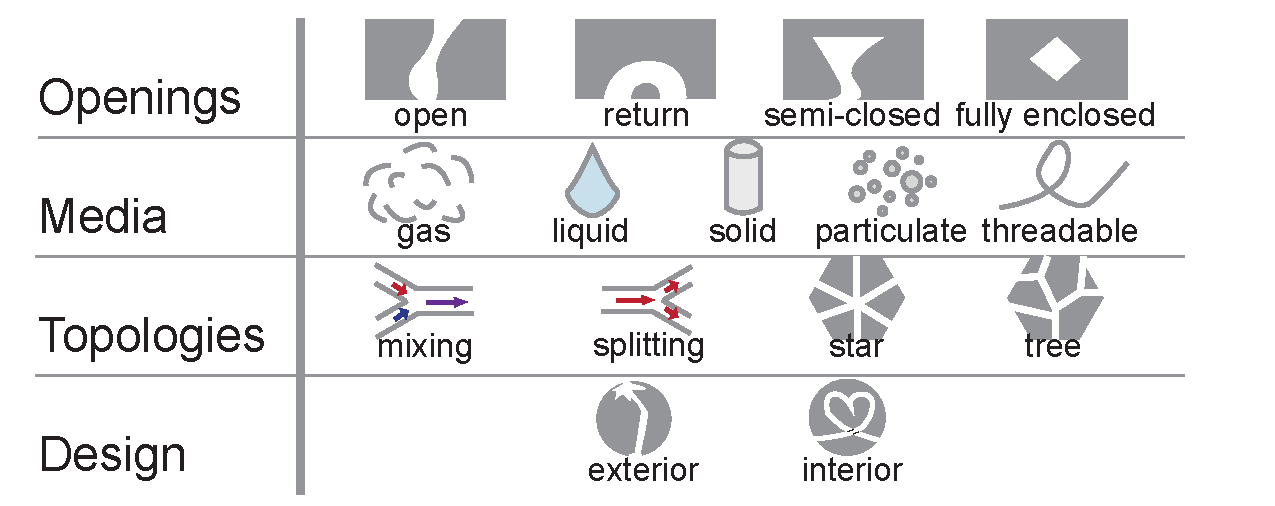
\includegraphics[width=3.4in]{figures/tubespace.pdf}
\caption{The design space of pipes.  Pipe types, media, topologies, and design are discussed more fully in the text.}
\label{fig:pipespace}
\end{figure}

\subsection{Openings of Pipes}

\tovi{this seems like a forced and
unnecessary definition. Do we really
need to distibguish the two ends?}
Pipes can come in four types: open, return, semi-closed, and fully enclosed.  Each of these types offers distinct interaction capabilities (see Figure \ref{fig:pipespace}).  Since we are interested in interactive devices, we distinguish a ``user side" - part of the surface or interior of an object facing its user; and a ``system side" - part of the object (either interior or exterior) where other hardware such as electronics will be connected.  Definitionally, in the following paragraphs we refer to a pipe which is ``open on the user side'' or ``open on the system side'' to have its contents \emph{physically accessible} to an interacting user or the system \emph{at interaction time}.  A pipe which is ``open on the user side'' or ``closed on the system side'' is physically cut off from the user or machine.  User and system manipulation of contents are possible with or without physical access, e.g., by resonating, pressurizing, or passing electricity through those contents.

\begin{figure}[h]
\centering
    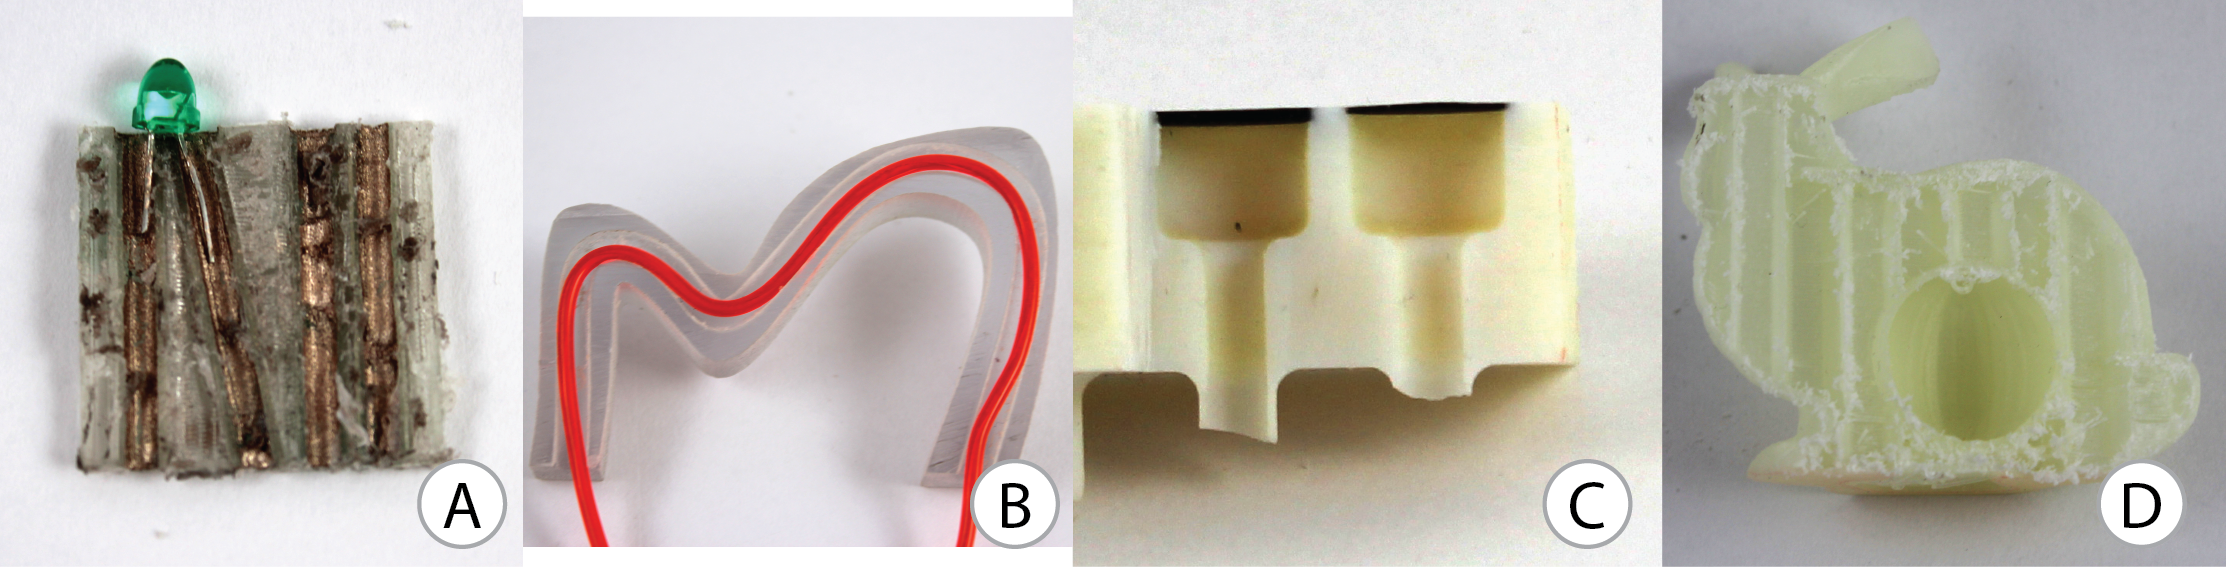
\includegraphics[width=3.4in]{figures/types.png}
\caption{Types of pipes.  A shows a pair of open tubes filled with copper paint to power an LED.  B shows a return pipe with EL wire threaded through it.  C shows two semi-closed pipes with rubber membranes at their ends.  In D, a rabbit has a fully enclosed chamber to modify its weight. \bjoern{Great, but make figure  full column wide}}
\label{fig:pipespace}
\end{figure}

Open pipes (see Figure \ref{fig:pipespace}A) originate from the system side and connect the user side, with both ends of the pipe open. This type of pipe may be used to create, for example, capacitive sensors: an open pipe filled with conductive paint can be connected to a sensing platform (e.g., Arduino) on the system side, while a user can touch the uncapped other end of the pipe.  Using Swept Frequency Capacitive Sensing \cite{Sato-touche} or other techniques, a user's touch of the open end can be sensed.  An open pipe can also be used for output, for example by creating in-air vortices as in \cite{Sodhi-aireal}.

A return pipe (see Figure \ref{fig:pipespace}B) originates at the system and returns back to it, without offering physical access to the user.  By threading an electroluminescent (EL) wire through a clear return pipe, a maker can create a custom piece of neon art.  If a return pipe passes very close to the surface of a 3D printed model, warm or cold water passed through the pipe could be used for temperature-based haptic feedback.

Semi-closed pipes (see Figure \ref{fig:pipespace}C) are open at the system end (for control of the enclosed medium) and closed at the user end.  The closed interface  may be fabricated from a malleable material: for example, a series of pipes terminated in thin rubber membranes on the user side can be actuated by an air pump to create haptic feedback, or a hinged cap can be blown open by air pressure.  Semi-closed pipes can also function as audio-generating resonance chambers.

A fully enclosed pipe (see Figure \ref{fig:pipespace}D) is closed to both the system side and the user side.  Fully enclosed pipes can be used as resonance chambers (e.g., for object identification), or as air bubbles (e.g., as used in Printed Optics (\cite{Willis-printedoptics}) for internal display).  They can also be used as containers for water or other particles that would otherwise fall out.

\subsection{Design of Pipes}
\tovi{This definition is a little bit vague.}
Pipe designs may emphasize either their exterior features (connection points) or their interior paths.  These two features lead to different kinds of interfaces.  An example interface that focuses on the exterior connection points is the touch sensitive toy in Figure \ref{fig:toys}, where pipes must exit the toy at the frontal lobe, parietal lobes, etc.  An interface focused on the internal path of the pipe is the neon sign in Figure \ref{fig:neon}: output is based on the shape of the pipe.

\subsection{Pipe Topologies}

Pipe network topologies enable different types of interactions.

Splitting or mixing pipes offer flexibility in output.  If a maker wished to create a painting device, she might wish to have two system-side pipes feeding in primary-colored red and blue paints which mix in varying ratios, allowing their pigments to combine before purple exits from the device (see Figure \ref{fig:pipespace}).  Splitting can also be useful, for example if our maker wants red paint output in two locations from her painting device, she could have one system-side pipe, but split the pipe into two (see Figure \ref{fig:pipespace}).  \bjoern{??}

Star and tree topologies are extensions of the splitting and mixing primitives, encompassing multiple-in and multiple-out in contrast to single-in/single-out.  Using a star topology in which the pipes were filled with conductive paint, we created toys with several touch-sensitive areas, see Figure \ref{fig:toys}. 

\subsection{Media in Pipes}

Pipes can be filled with a variety of media to create different interface affordances and capabilities.

``Gas'' comprises all compressible fluids.  Fluid pressure inside semi-closed pipes can create haptic feedback, or gases can be used as carriers for scents or fog.  Slyper, et al.,  in \cite{Slyper-pressure} engineered structures to change in air pressure when manipulated correctly (e.g., a spiral that changes pressure when twisted, but not when pressed); fluid pressure can also be used as an input.

Incompressible fluids (``liquids'') can perform many of the same interface tasks as gases.  One opportunity with liquids is to fill the interior of pipes with them and cap the ends.  In addition, one can use driable conductive fluids, such as copper paint, to coat the interior of pipes and allow them to function as arbitrarily-shaped wires.  This is especially helpful for the creation of a shared ground, or for creating single-wire capacitive interfaces amenable to sensing with SFCS \cite{Sato-touche}.

Pipes need not have hollow centers: in the case where routed pipes are filled with solid material---in particular, a solid material different from the model material---, interactions such as those in Printed Optics (\cite{Willis-printedoptics}) are possible.

Particulates, either printed in-place or inserted, can be of varying densities.  A single particle can be used for display.  Sparse particles in a stream of fluid can provide haptic feedback.  Dense particles in a semi-closed pipe capped with flexible surface material allow for jamming-based interactions at any point on the surface of an object \cite{Follmer-jamming}; when fluid pressure in the pipe is reduced, the trapped particles jam to form a solid mass the same shape as their enclosing flexible membrane.

Threadable inserted elements, such as electroluminescent (EL) wire or fiberoptic cables, are those that can be threaded through pipes post-printing.  This allows overcoming limitations of printers: for example, a Printed Optics-style interface can be created on an inexpensive consumer-grade 3D printer using pipes and inserted fiber optic cable.